% !TeX root = ./eLife_draft.tex

%%%%%%%%%%%%%%%%%%%%%%%%%%%%%%%%%%%%%%%%%%%%%%%%%%%%%%%%%%%%
%%% ELIFE ARTICLE TEMPLATE
%%%%%%%%%%%%%%%%%%%%%%%%%%%%%%%%%%%%%%%%%%%%%%%%%%%%%%%%%%%%
%%% PREAMBLE 
\documentclass[9pt,lineno]{elife}
% Use the onehalfspacing option for 1.5 line spacing
% Use the doublespacing option for 2.0 line spacing
% Please note that these options may affect formatting.
% Additionally, the use of the \newcommand function should be limited.

\usepackage{lipsum} % Required to insert dummy text
\usepackage[version=4]{mhchem}
\usepackage{siunitx}
\DeclareSIUnit\Molar{M}

%%%%%%%%%%%%%%%%%%%%%%%%%%%%%%%%%%%%%%%%%%%%%%%%%%%%%%%%%%%%
%%% ARTICLE SETUP
%%%%%%%%%%%%%%%%%%%%%%%%%%%%%%%%%%%%%%%%%%%%%%%%%%%%%%%%%%%%

\title{Fundamental limits on the rate of bacterial cell division}
\author[1, *]{Nathan M. Belliveau}
\author[2, 3, *]{Griffin Chure}
\author[4]{Christina L. Hueschen}
\author[5]{Hernan G. Garcia}
\author[6]{Jan\'{e} Kondev}
\author[7]{Daniel S. Fisher}
\author[1, 8]{Julie Theriot}
\author[1, 9, $\dagger$]{Rob Phillips}
\affil[1]{Department of Biology, University of Washington, Seattle, WA, USA}
\affil[2]{Division of Biology and Biological Engineering, California Institute of Technology, Pasadena, CA, USA}
\affil[3]{Department of Applied Physics, California Institute of Technology, Pasadena, CA, USA}
\affil[4]{Department of Chemical Engineering, Stanford University, Stanford, CA, USA}
\affil[5]{Department of Molecular Cell Biology and Department of Physics, University of California Berkeley, Berkeley, CA, USA}
\affil[6]{Department of Physics, Brandeis University, Waltham, MA, USA}
\affil[7]{Department of Applied Physics, Stanford University, Stanford, CA, USA}
\affil[8]{Allen Institute for Cell Science, Seattle, WA, USA}
\affil[9]{Department of Physics, California Institute of Technology, Pasadena, CA, USA}
\affil[$\dagger$]{Address correspondence to phillips@pboc.caltech.edu}
\affil[*]{Contributed equally}

\contrib[$\dagger$]{These authors contributed equally to this work}

%%%%%%%%%%%%%%%%%%%%%%%%%%%%%%%%%%%%%%%%%%%%%%%%%%%%%%%%%%%%
%%% ARTICLE START
%%%%%%%%%%%%%%%%%%%%%%%%%%%%%%%%%%%%%%%%%%%%%%%%%%%%%%%%%%%%

\begin{document}

\maketitle

\begin{abstract}

\end{abstract}

\section{Introduction}

The intimate relationship between the environment and cellular growth rate
has remained a major topic of inquiry in bacterial physiology for over a
century. 

\begin{figure}
    \centering{
    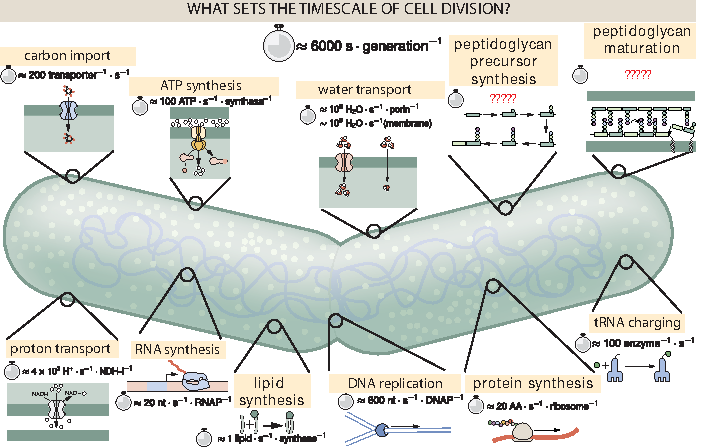
\includegraphics{../../figures/categories.pdf}
    \caption{\textbf{Transport and synthesis processes necessary for cell division.}}
    \label{fig:categories}
    }
\end{figure}



Points to emphasize
\begin{itemize}
\item The past decade of work in proteomics has made high-througput absolute
measurement of protein abundance a reality. Recent groups have used mass
spectrometry and ribosomal profiling to quantify growth-dependent effects on
protein copy numbers across growth conditions. In this work, we assemble four
recent datasets that examine how cellular proteome is influenced by the total
growth rate. 
\end{itemize}
% \section{Transport of Biochemical Building Blocks}
We begin with an interrogation of some of the myriad transport systems bacteria
use to bring extracellular materials (such as carbon, water, and ions) into the
cell. 

\subsection{Carbon Transport}
All macromolecules synthesized by cells include carbon as the primary elemental 
constituent. It is therefore reasonable to consider the acquisition of carbon
from the environment, typically in the form of sugar, as a candidate process 
which sets the bacterial speed limit. We can a combination of biological intuition
and the vast literature on the molecular composition of \textit{E. coli} to make 
an order-of-magnitude estimate for the total number of sugar transporters needed 
double. 

For convenience, we will consider a condition in which glucose is the primary
carbon source in a growth medium. In standard laboratory conditions, a
minimal medium supplemented with only glucose will have a growth rate of
$\approx 1 \text{generation}\cdot\text{hr}^{-1}$ which is an approximate
doubling time of $\approx 3000 $ seconds. During this time, the cell must be
able to import enough carbon molecules to double all macromolecules.  

We can begin by using the well justified estimate that the typical \textit{E. coli}
cell is $\approx$ 70\% water by mass, yielding a $\approx$ 30\% dry mass (BNID: 109049, \cite{milo2010}).
Exponential growth of \textit{E. coli} in a glucose based medium results in an 
average cell volume of 1 fL, bringing our total dry mass to 30 pg. Assuming half of 
this dry mass is protein (0.15 pg), we can estimate how many carbons are present in 
the protein pool.   

Let's assume that a standard protein is approximately 300 amino acids long,
which comes out a mass of $\approx$ 30 kDa. From this, we estimate that the
total number of amino acids (incorporated into protein) is
\begin{equation}
    N_\text{AA} = \left(1.5 \times 10^{-13}\,\text{g}\right) \times
\left({1\,\text{protein} \over 3 \times 10^4\, \text{Da}}\right) \times
\left( {6 \times 10^{23}\,\text{Da} \over 1\,\text{g}}\right) \times \left({3
\times 10^2 \,\text{AA} \over \text{protein}}\right) \approx 2.5 \times
10^8\,\text{Amino\, Acids}. 
\label{eq:num_amino_acids}
\end{equation}
The typical amino acid consists of a two-carbon backbone with a $\approx$ 3
carbon side-chain. Thus, assuming the typical amino acid contains $\approx$ 5
carbons, the total mass of carbon in the protein pool can be calculated as
\begin{equation}
    N_\text{C}^\text{(protein)} = N_\text{AA} \times {\text{C} \over \text{AA}}
= 2.5 \times 10^8\, \text{AA} \times {5\, \text{C} \over \text{AA}} \approx 5
\times 10^9\, {\text{C} \over \text{cell}}. 
\label{eq:n_carbon_protein}
\end{equation}
Since we approximated that about half of the dry mass is protein, it's
reasonable to assume that the remaining half of the dry mass has a similar
composition, permitting us to say that
\begin{equation}
N_\text{C}^{\text{(cell)}} \approx 2 \times N_\text{C}^\text{(protein)} =
10^{10} {\text{C} \over \text{cell}}. 
\label{eq:n_carbon_cell}
\end{equation}
With a handle on the total number of carbons needed per cell, we can now try
to estimate how many sugar transporters would be needed to transport 100
billion carbon atoms per standard cell doubling time of $\approx 3000$ seconds. With 6
carbon atoms per glucose molecule, we can estimate the minimum glucose flux
across the membrane to be
\begin{equation}
J_\text{glucose} = {10^{10}\,\text{C} \over \text{cell}} \times {1\,
\text{glucose} \over 6\, \text{C}} \times {1\,\text{cell} \over 3 \times
10^3\,\text{s}} \approx 5 \times 10^6 {\text{glucose} \over \text{s}}.
\label{eq:glucose_flux}
\end{equation}
The chief glucose transport system of \textit{E. coli} (the PTS system) can 
transport $\approx 200\, \text{glucose}\cdot\text{s}^{-1}$ (BNID: 103693 \cite{milo2010})
meaning that the \textit{minimum} number of glucose transporters per cell needed 
to double the cellular carbon content is
\begin{equation}
N_\text{tpr.} \approx {J_\text{glucose} \over J_\text{transporter}} = {5
\times 10^6 \text{glucose / s} \over 2 \times 10^2 \,\text{glucose / s}}
\approx 2 \times 10^4\, \text{tpr. / cell}.
\label{eq:n_gluc_transporters}
\end{equation}




\subsection{Water Transport}
% \section{Energy Production}

While the transport of nutrients is required to build new cell mass, the
metabolic pathways both consume and generate energy
in the form of NTPs. The high-energy phosophodiester bonds of (primarily) ATP
power a variety of cellular processes that drive biological systems away
from thermodynamic equilibrium. The next set of processes we hypothesize might
control the rate of cell division considers the energy budget
of a dividing cell in terms of the synthesis of ATP from ADP and inorganic
phosphate as well as maintenance of the electrochemical proton gradient which powers it.

\subsection{ATP Synthesis}

Hydrolysis of the terminal phosphodiester bond of ATP forming ADP and an
inorganic phosphate is a kinetic driving force in a wide array of biochemical
reactions. One such reaction is the formation of peptide bonds during
translation which requires $\approx$ 2 ATPs for the charging of an amino acid
to the tRNA and $\approx$ 2 ATP equivalents for the formation of the peptide
bond between amino acids. Considering the ATP costs associated with error
correction and post-translational modifications of proteins, we can make the
approximation that each peptide bond has a net cost of $\approx$ 5 ATP (BNID:
107782, \cite{milo2010}). In total, the energetic costs of peptide bond
formation consume $\approx$
80\% of the cells ATP budget (BNID: 107782; 106158; 101637; 111918,
\cite{milo2010, lynch2015,stouthamer1973}). The pool of ATP is produced by
the F$_1$-F$_0$ ATP synthase
-- a membrane-bound rotary motor which under ideal conditions can yield
$\approx$ 300 ATP per second (BNID: 114701; \cite{milo2010, weber2003}).

To estimate the total number of ATP equivalents consumed during a cell cycle,
we will make the approximation that there are $\approx 3\times10^6$ proteins
per cell with an average protein length of $\approx$ 300 peptide bonds (BNID:
115702; 108986; 104877, \cite{milo2010}). Taking these values together, we
estimate that the typical \textit{E. coli} cell consumes $\approx 5 \times
10^9$ ATP per cell cycle on protein synthesis alone and $\approx 6\times
10^9$ ATP in total. Assuming that the ATP synthases are operating at their
fastest possible rate, $\approx$ 3000 ATP synthases are needed to keep up
with the energy demands of the cell. This estimate and a comparison with the
data are shown in \FIG{energy_production} (A). Despite our assumption of
maximal ATP production rate per synthase and approximation of all NTP
consuming reactions being the same as ATP, we find that an estimate of a few
thousand complete synthases per cell to agree well with the experimental
data. Much as we did for the estimates of transporter copy number in the
previous section, we can
generalize this estimation to consider a continuum of growth rates rather than a
point estimate of 5000 s, indicated by the gray lines in
\FIG{energy_production}, and find that this approach adequately describes the
observed growth rate dependence. 

If the direct production of ATP was a rate limiting step for
growth, could the cell simply express more ATP synthase complexes? This
requires us to consider several features of cellular physiology, namely the
physical space on the inner membrane as well as the ability to maintain the
proton chemical gradient leveraged by the synthase to drive ATP production
out of equilibrium.

\subsection{Generating the Proton Electrochemical Gradient}
In order to produce ATP, the F$_1$-F$_0$ ATP synthase itself must consume
energy. Rather than burning through its own product, this intricate
macromolecular machine has evolved to exploit the electrochemical potential
established across the inner membrane through cellular respiration. This
electrochemical gradient is manifest  by the pumping of protons into the
intermembrane space via the electron transport chains as they reduce NADH. In
\textit{E. coli}, this potential difference is $\approx -$200 mV (BNID: 102120,
\cite{milo2010}). A simple estimate of the inner membrane as a capacitor with a
working voltage of -200 mV (as performed in the Supplemental Information)
reveals that $\approx 2\times 10^4$ protons must be present in the intermembrane space.

However, the constant rotation of the ATP synthases would rapidly abolish
this potential difference if it were not being actively maintained. To
undergo a complete rotation (and produce a single ATP), the F$_1$-F$_0$ ATP
synthase must shuttle $\approx$ 4 protons across the membrane into the
cytosol (BNID: 103390, \cite{milo2010}). With $\approx$ 3000 ATP synthases each
generating 300 ATP per second, the $2 \times 10^4$ protons establishing the 200
mV potential would be consumed in only a few milliseconds. This brings us
to our next estimate: how many electron transport complexes are needed to
support the consumption rate of the ATP synthases?

The electrochemistry of the electron transport complexes of \textit{E. coli}
have been the subject of intense biochemical and biophysical study over the past
half century \citep{ingledew1984, khademian2017,cox1970,henkel2014}. A recent
work \citep{szenk2017} examined the respiratory capacity of the \textit{E. coli}
electron transport complexes using structural and biochemical data, revealing
that each electron transport chain rapidly pumps protons into the intermembrane
space at a clip of $\approx$ 1500 protons per second (BIND: 114704; 114687,
\cite{milo2010}). Using our estimate of the number of ATP synthases required per
cell (\FIG{energy_production}(A)), coupled with these recent measurements, we
estimate that $\approx 1000$ electron transport complexes would be necessary to
facilitate the $\approx 4\times 10^6$ protons per second diet of the cellular
ATP synthases. This estimate (along with a generalization to the entire range of
observed growth rates) is in agreement with the number of complexes
identified in the proteomic datasets (plot in \FIG{energy_production}(B)). This
suggests that every ATP synthase must be accompanied by $\approx$ 1 functional
electron transport chain. Again, if this were a rate limiting process for
bacterial growth, one must conclude that it is not possible for the cell to
simply increase the production of both the number of electron transport chain
complexes as well as ATP synthases. As both of these components only function
bound to the inner membrane, we now turn our attention towards the available
space in the membrane as well as surface-area-to-volume constraints.


\begin{figure}
    \begin{fullwidth}
        \centering{
            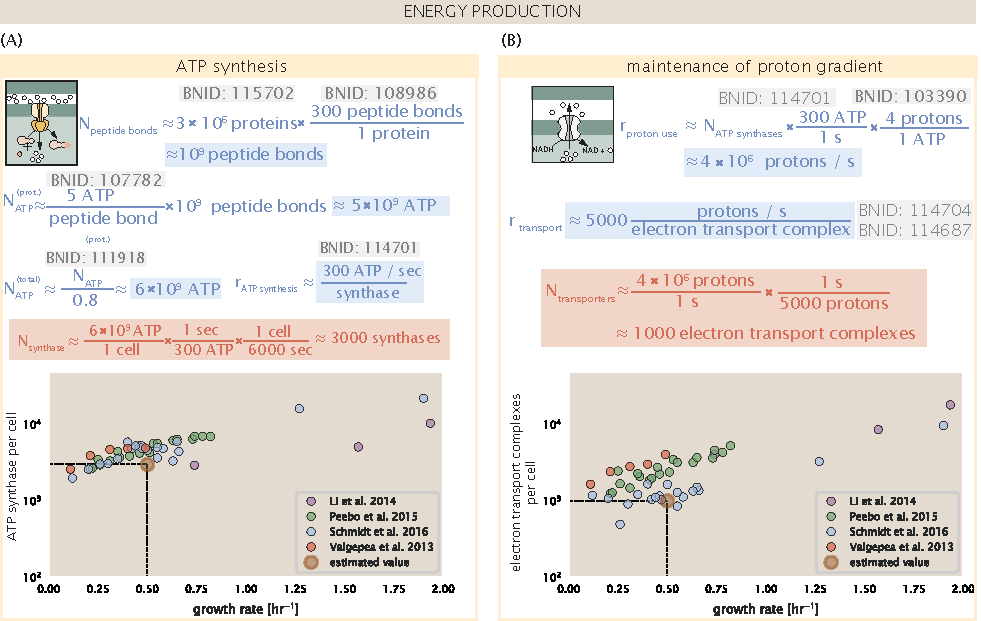
\includegraphics{main_figs/fig4_energy_production.pdf}
            \caption{\textbf{The abundance of F$_1$-F$_0$ ATP synthases and
            electron transport chain complexes as a function of growth
            rate.} (A) Estimate of the number of F$_1$-F$_0$ ATP synthase
            complexes needed to accommodate peptide bond formation and other NTP
            dependent processes. Points in plot correspond to the
            mean number of complete F$_1$-F$_0$ ATP synthase complexes that
            can be formed given proteomic measurements and the subunit
            stoichiometry
            [AtpE]$_{10}$[AtpF]$_2$[AtpB][AtpC][AtpH][AtpA]$_{3}$[AtpG][AtpD]$_3$.
            (B) Estimate of the number of electron transport chain complexes
            needed to maintain a membrane potential of $-$200 mV given
            estimate of number of F$_1$-F$_0$ ATP synthases from (A). Points
            in plot correspond to the average number of complexes identified
            as being involved in aerobic respiration by the Gene Ontology
            identifier GO:0019646 that could be formed given proteomic
            observations. These complexes include cytochromes \textit{bd1}
            ([CydA][CydB][CydX][CydH]), \textit{bdII} ([AppC][AppB]),
            \textit{bo$_3$},([CyoD][CyoA][CyoB][CyoC]) and NADH:quinone
            oxioreducase I
            ([NuoA][NuoH][NuoJ][NuoK][NuoL][NuoM][NuoN][NuoB][NuoC][NuoE][NuoF][NuoG][NuoI])
            and II ([Ndh]). Grey lines in both (A) and (B) correspond to the
            estimate procedure described, but applied to a continuum of growth
            rates. We direct the reader to the Supporting Information for a more
            thorough description of this approach.}
        \label{fig:energy_production}
        }
    \end{fullwidth}
\end{figure}


\subsection{Energy Production in a Crowded Membrane.}

For each protein considered so far, the data shows that in general their numbers
increase with growth rate. This is in part a consequence of the increase in cell
length and width at that is common to many rod-shaped bacteria at faster growth
rates \citep{ojkic2019, harris2018}. For the particular case of \textit{E.
coli}, the total cellular protein and cell size increase logarithmically with
growth rate \citep{schaechter1958, si2017}. Indeed, this is one reason why we
have considered only a single, common growth condition across all our estimates
so far. Such a scaling will require that the total number of proteins and net
demand on resources also grow in proportion to the increase in cell size divided
by the cell's doubling time. Recall however that each transport process, as well
as the ATP production via respiration, is performed at the bacterial membrane.
This means that their maximum productivity can only increase in proportion to
the cell's surface area divided by the cell doubling time. This difference in
scaling would vary in proportion to the surface area-to-volume (S/V) ratio.

While we found that there was more than sufficient membrane real estate for
carbon intake in our earlier estimate, the total number of ATP synthases and
electron chain transport complexes both exhibit a clear increase in copy number
with growth rate, reaching in excess of 10$^4$ copies per cell
(\FIG{energy_production}). Here we consider the consequences of this
S/V ratio scaling in more detail.

In our estimate of ATP production above we found that a cell demands about
$6 \times 10^9$ ATP or $10^6$ ATP/s. With a cell volume of roughly 1 fl, this
corresponds to about $2 \times 10^{10}$ ATP per fL of cell volume, in line  with
previous estimates \citep{stouthamer1977, szenk2017}. In \FIG{energy_scaling} (A)
we plot this ATP demand as a function of the S/V ratio in green, where we have
considered a range of cell shapes from spherical to rod-shaped with an aspect
ratio (length/width) equal to 4 (See appendix for calculations of cell volume
and surface area).  In order to consider the maximum power that could be
produced, we consider the amount of ATP that can generated by a membrane filled
with ATP synthase and electron transport complexes, which provides a maximal
production of about 3 ATP / (nm$^2 \cdot$s) \citep{szenk2017}. This is shown in
blue in \FIG{energy_scaling}(A), which shows that at least for the growth rates
observed, the energy demand is roughly an order of magnitude less.  

Interestingly, \cite{szenk2017} also found that ATP production by
respiration is less efficient than by fermentation per membrane area occupied
due to the additional proteins of the electron transport chain. This suggests
that even under anaerobic growth, there will be sufficient membrane space for
ATP production in general.

While this serves to highlight the diminishing capacity to provide resources to
grow if the cell increases in size (and its S/V decreases), the blue region in
\FIG{energy_scaling}(A) represents a somewhat unachievable limit since the inner
membrane must also include other proteins such as those required for lipid and
membrane synthesis. To gain insight, we used the proteomic data
to look at the distribution of proteins on the inner membrane. Here we use Gene
Ontology (GO) annotations \citep{ashburner2000,thegeneOntologyconsortium2018} to
identify all proteins embedded or peripheral to the inner membrane (GO term:
0005886). Those associated but not membrane-bound include proteins like MreB and
FtsZ, that traverse the inner membrane by treadmilling and must nonetheless be
considered as a vital component occupying space on the membrane. In
\FIG{energy_scaling} (B), we find that the total protein mass per $\mu$m$^2$ is
relatively constant with growth rate. Interestingly, when we consider the
distribution of proteins grouped by their Clusters of Orthologous Groups (COG)
\citep{tatusov2000}, the relative abundance for those in metabolism
(including ATP synthesis via respiration) is also relatively constant.

\begin{figure}
    \begin{fullwidth}
        \centering{
            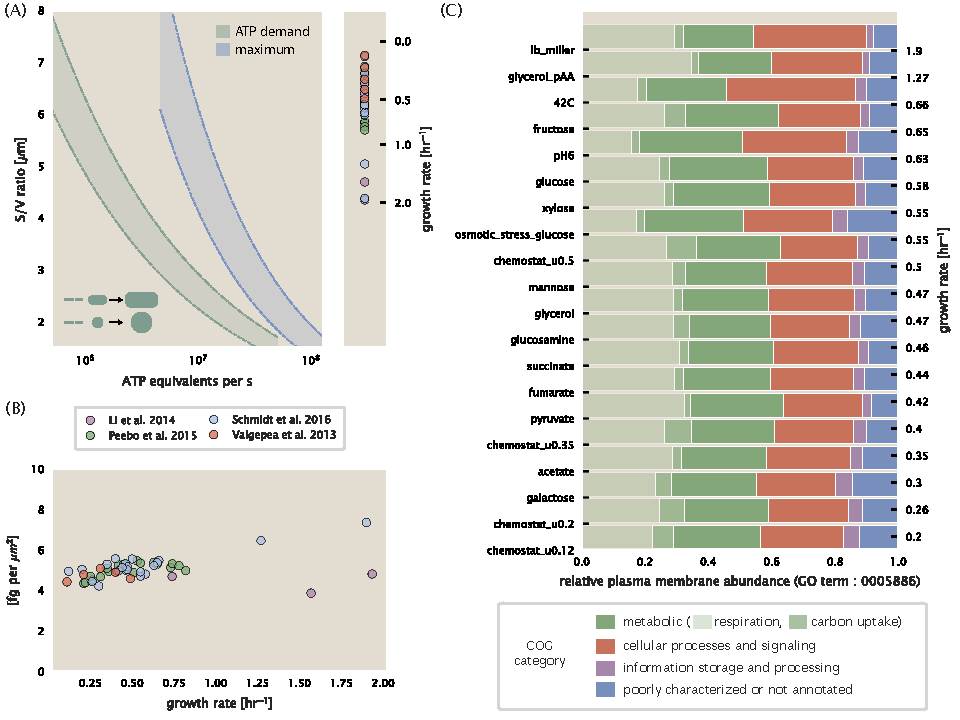
\includegraphics{main_figs/fig5_energy_SV_scaling.pdf}
            \caption{\textbf{Influence of cell size and S/V ratio on ATP
            production and inner membrane composition.} (A) Scaling of ATP
            demand and maximum ATP production as a function of S/V ratio.
            Cell volumes of 0.5 fL to 50 fL were considered, with the dashed
            (\texttt{- -})
            line corresponding to a sphere and the
            dash-dot line (\texttt{-.}) reflecting a rod-shaped bacterium like \textit{E.
            coli} with a typical aspect ratio (length / width) of 0.4 \citep{shi2018}. Approximately 50\% of the bacterial inner
            membrane is assumed to be protein, with the remainder lipid. (B)
            Total protein mass calculated for proteins with inner membrane
            annotation (GO term: 0005886). (C) Relative protein abundances by
            mass based on COG annotation. Metabolic proteins are further
            separated into respiration (F$_1$-F$_0$ ATP synthase, NADH
            dehydrogenase I, succinate:quinone oxidoreductase, cytochrome
            bo$_3$ ubiquinol oxidase, cytochrome bd-I ubiquinol oxidase) and
            carbohydrate transport (GO term: GO:0008643). Note that the
            elongation factor EF-Tu can also associate with the inner
            membrane, but was excluded in this analysis due to its high
            relative abundance (roughly identical to the total mass shown in
            part (B)).}
        \label{fig:energy_scaling}
        }
    \end{fullwidth}
\end{figure}



% \begin{table}[bt]
% \caption{\label{tab:example}Automobile Land Speed Records (GR 5-10).}
% % Use "S" column identifier to align on decimal point 
% \begin{tabular}{S l l l r}
% \toprule
% {Speed (mph)} & Driver          & Car                        & Engine    & Date     \\
% \midrule
% 407.447     & Craig Breedlove & Spirit of America          & GE J47    & 8/5/63   \\
% 413.199     & Tom Green       & Wingfoot Express           & WE J46    & 10/2/64  \\
% 434.22      & Art Arfons      & Green Monster              & GE J79    & 10/5/64  \\
% 468.719     & Craig Breedlove & Spirit of America          & GE J79    & 10/13/64 \\
% 526.277     & Craig Breedlove & Spirit of America          & GE J79    & 10/15/65 \\
% 536.712     & Art Arfons      & Green Monster              & GE J79    & 10/27/65 \\
% 555.127     & Craig Breedlove & Spirit of America, Sonic 1 & GE J79    & 11/2/65  \\
% 576.553     & Art Arfons      & Green Monster              & GE J79    & 11/7/65  \\
% 600.601     & Craig Breedlove & Spirit of America, Sonic 1 & GE J79    & 11/15/65 \\
% 622.407     & Gary Gabelich   & Blue Flame                 & Rocket    & 10/23/70 \\
% 633.468     & Richard Noble   & Thrust 2                   & RR RG 146 & 10/4/83  \\
% 763.035     & Andy Green      & Thrust SSC                 & RR Spey   & 10/15/97\\
% \bottomrule
% \end{tabular}

% \tabledata{This is a description of a data source.}

% \end{table}







% For a half-width figure or table with text wrapping around it, use 

% \begin{verbatim}
% \begin{wrapfigure}{l}{.46\textwidth}
%   \includegraphics[width=\hsize]{...}
%   \caption{...}\label{...}
% \end{wrapfigure}
% \end{verbatim}
% %
% as in \FIG{halfwidth}. For tables:

% If you use the following prefixes for your \verb|\label|:
% %
% \begin{description}
% \item[Figures] \texttt{fig:}, e.g.~\verb|\label{fig:view}|
% \item[Figure Supplements] \texttt{figsupp:}, e.g.~\verb|\label{figsupp:sf1}|\\
% (we'll assume \texttt{figsupp:sf1} is a figure supplement of \texttt{fig:view} in our example)
% \item[Figure source data] \texttt{figdata:}, e.g.~\verb|\label{figdata:first}|
% \item[Videos] \texttt{video:}, e.g.~\verb|\label{video:mv1}|
% \item[Video supplements] \texttt{videosupp:}, e.g.~\verb|\label{videosupp:sv1}|
% \item[Tables] \texttt{tab:}, e.g.~\verb|\label{tab:example}|
% \item[Equations] \texttt{eq:}, e.g.~\verb|\label{eq:CLT}|
% \item[Boxes] \texttt{box:}, e.g.~\verb|\label{box:simple}|
% \end{description}
% %
% you can then use the convenience commands \verb|\FIG{view}|, \verb|\FIGSUPP[view]{sf1}|, \verb|\TABLE{example}|, \verb|\EQ{CLT}|, \verb|\BOX{simple}|, \verb|\FIGDATA[view]{first}|, \verb|\VIDEO{mv1}| and \verb|{\VIDEOSUPP}[view]{sv1}| \emph{without} the label prefixes, to generate cross-references \FIG{view}, \FIGSUPP[view]{sf1},  \TABLE{example}, \EQ{CLT}, \BOX{simple}, \FIGDATA[view]{first}, \VIDEO{mv1} and \VIDEOSUPP[view]{sv1}. Alternatively, use \verb|\autoref| with the full label, e.g.~\autoref{first:app} (although this may not work correctly for figures and tables in the appendices or boxes nor supplements at present).

% Really wide figures or tables, that take up the entire page, including the gutter space: use \verb|\begin{fullwidth}...\end{fullwidth}| as in \FIG{fullwidth}. And sometimes you may want to use feature boxes like \BOX{simple}.

% \begin{wrapfigure}{l}{.46\textwidth}
% \includegraphics[width=\hsize]{frog}
% \caption{A half-columnwidth image using wrapfigure, to be used sparingly. Note that using a wrapfigure before a sectional heading, near other floats or page boundaries is not recommended, as it may cause interesting layout issues. Use the optional argument to wrapfigure to control how many lines of text should be set half-width alongside it.}
% \label{fig:halfwidth}
% \end{wrapfigure}


% \begin{figure}
% \begin{fullwidth}
% \includegraphics[width=0.95\linewidth]{elife-18156-fig2}
% \caption{A very wide figure that takes up the entire page, including the gutter space.}
% \label{fig:fullwidth}
% \figsupp{There is no limit on the number of Figure Supplements for any one primary figure. Each figure supplement should be clearly labelled, Figure 1--Figure Supplement 1, Figure 1--Figure Supplement 2, Figure 2--Figure Supplement 1 and so on, and have a short title (and optional legend). Figure Supplements should be referred to in the legend of the associated primary figure, and should also be listed at the end of the article text file.}{\includegraphics[width=5cm]{frog}}
% \end{fullwidth}
% \end{figure}


% \figsupp[Shorter caption for main text.]{This is a supplementary figure's full caption, which will be used at the end of the manuscript.}{\includegraphics[width=6cm]{frog}}\label{figsupp:sf1}
% \figsupp{This is another supplementary figure.}{\includegraphics[width=6cm]{frog}}
% \videosupp{This is a description of a video supplement.}\label{videosupp:sv1}
% \figdata{This is a description of a data source.}\label{figdata:first}
% \figdata{This is another description of a data source.}\label{figdata:second}






% \section{Acknowledgments}

% Additional information can be given in the template, such as to not include funder information in the acknowledgments section.

% \nocite{*} % This command displays all refs in the bib file. PLEASE DELETE IT BEFORE YOU SUBMIT YOUR MANUSCRIPT!
\bibliography{library.bib}

%%%%%%%%%%%%%%%%%%%%%%%%%%%%%%%%%%%%%%%%%%%%%%%%%%%%%%%%%%%%
\end{document}